\section{Theoretical background}

\subsection{Markov Decision Processes}

Markov Decision Processes (MDPs) are a classical formalization of sequential decision making, where actions influence not just immediate rewards, but also subsequent situations (states) and through those future rewards. Thus MDPs involve delayed reward and the need to tradeoff immediate and delayed reward.

A Markov Decision Process consists of a set of states $S$ and a set of actions $A$. The dynamics of the MDP, from any state $s \in S$ and for any action $a \in A$, are determined by transition probabilities, $P^a_{ss'} = Pr(s_{t+1} = s' | s_t = s, a_t = a)$, specifying the distribution over the next state $s' \in S$. Finally, a reward function, $R^a_{ss'} = \EX[r_{t+1} | s_t = s, a_t = a, s_{t+1} = s']$, specifies the expected reward for a given state transition.
Episodic MDPs terminate with probability 1 in a distinguished terminal state, $s_T \in S$, after finite number of transitions. Continuous MDPs doesn't include the terminal state and can run endlessly.
The return $R_t = \sum^T_{k=t}r_k$ is the total reward accumulated in that episode from time $t$ until reaching the terminal state at time $T$. In continuous MDPs this is the sum of an infinite sequence of rewards from time $t$.
A policy, $\pi(s, a) = Pr(a_t = a | s_t = s)$, maps a state $s$ to a probability distribution over actions.
The value function, $V_\pi(s) = \EX_\pi[R_t | s_t = s]$, is the expected return from state $s$ when following policy $\pi$.
The action value function, $Q_\pi(s, a) = \EX_\pi[R_t | s_t = s, a_t = a]$, is the expected return after selecting action $a$ in state $s$ and then following policy $\pi$.
The optimal value function is the unique value function that maximises the value of every state, $V^*(s) = maxV_\pi(s), \forall_{s \in S}$ and $Q^*(s, a) = maxQ_\pi(s, a), \forall_{s \in S, a \in A}$. An optimal policy $\pi^*(s, a)$ is a policy that maximises the action value function from every state in the MDP, $\pi^*(s, a) = \underset{a}{\mathrm{argmax}}Q^*(s, a)$.

MDPs are a mathematically idealized form of the reinforcement learning problem for which precise theoretical statements can be made. In reinforcement learning the dynamics and the reward function are hidden behind an environment. Consequently, we can't directly use them for planning, but we can learn through interaction with the environment.

\subsection{Reinforcement Learning}

Reinforcement learning (RL) is learning what to do, how to map situations to actions, so as to maximize a numerical reward signal.\cite{Book.RLAI} This mapping is called a policy $\pi$. RL consists of an agent that, in order to learn a good policy, acts in an environment. The environment provides a response to each agent's action $a$ that is interpreted and fed back to the agent. Reward $r$ is used as a reinforcing signal and state $s$ is used to condition agent's decisions. Fig.~\ref{Fig.RL} explains it in the diagram.
Each action-response-interpretation sequence is called a step or a transition. Multiple steps form an episode. The episode finishes in a terminal state $s_T$ and the environment is reset in order to start the next episode from scratch. Very often, RL agents need dozens and dozens of episodes to gather enough experience to learn the (near) optimal policy.

\begin{figure}[H]
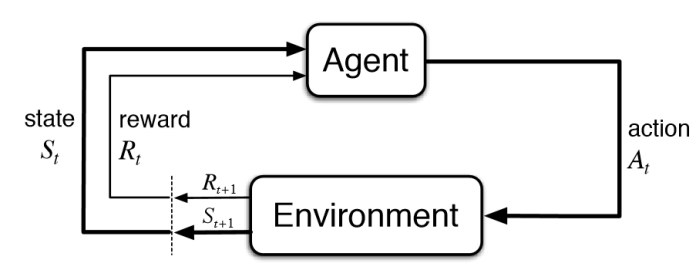
\includegraphics[]{figures/RL.jpg}
\caption{Reinforcement Learning\protect\cite{Book.RLAI}}
\label{Fig.RL}
\end{figure}

\editnote{Should I describe here General Policy Iteration, Monte-Carlo Control, TD-Learning, ... what else? Rather than guessing what needs to be described, continue work and see what needs more attention.}

\subsection{Deep Learning}

It's like Machine Learning... but deeper.

\begin{figure}[H]

\includegraphics[width=0.8\textwidth,keepaspectratio]{figures/DL.jpg}
\caption{Deep Learning}
\label{Fig.DL}
\end{figure}
